\section{Learning Algorithms}
\label{sec:learning}

After extracting the feature vectors, we can train the classifier for instance matching. There are many machine learning algorithms for the binary classification problem. We need to carefully choose the appropriate ones according to the characteristic of the input data.

\subsection{Basic Learning Model}

In our problem, the input data may contain millions instance pairs. So some methods with high time cost such as \textit{Neural Networks} and \textit{SVM} with a complex kernel are eliminated. After observing the feature space via a preliminary experiment, we found that the data of the two classes are not linearly separable. A typical example is shown in Figure \ref{fig:space}. $x$ and $y$ are two dimensions of the similarity vector. The positive and negative regions represent the two classes. Figure \ref{fig:space} indicates that for a similarity vector, if $x$ is greater than a threshold, it belongs to the class of matching instance pairs when $y$ is large, but if $x$ is less than the threshold, it belongs to the matching class when $y$ is small. From the perspective of each single dimension, this situation does not meet our intuition. The value of each dimension describes the similarity of two instances based on a certain metric. The higher the value is, the more likely they will match. But from the perspective of the correlation between the dimensions, such a situation is reasonable. We will give an example to explain it.

\begin{figure}[t]
  \centering
  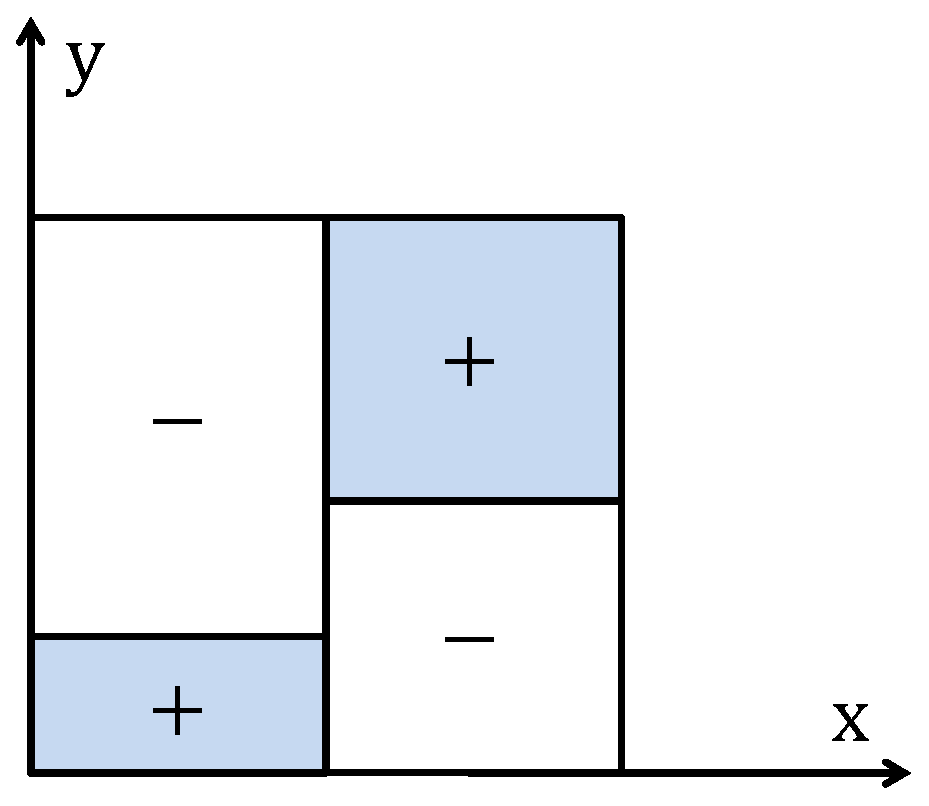
\includegraphics[width=0.3\textwidth]{figures/space}
  \caption{A typical example of the feature space}
  \label{fig:space}
\end{figure}

On one hand, given two instance pairs $(p_1, p_2)$ and $(q_1, q_2)$, their similarity vectors are $u$ and $v$. We assume that $u_6=v_6=0.3$, $u_5=0.1$ and $v_5=0.3$ where $u_i$($v_i$) stands for the $i$th dimension of the similarity vector $u$($v$). Probably, instance $p_1$ consists of long texts and instance $p_2$ consists of short texts or single words, so that $u_5=0.1$. While $q_1$ and $q_2$ both consist of long texts which share some common (for the domain) words, so $v_5=0.3$. Furthermore, $p_1$ and  $p_2$ may share some important words such that $u_6=0.3$. While the value $0.3$ of $v_6$ may be obtained by the common words. According to the inference above, $(p_1, p_2)$ is likely to match while $(q_1, q_2)$ is not. On the other hand, an instance pair with large values of both dimensions $5$ and $6$ is likely to match.

Since the feature space is so complex, some linear classifiers are inapplicable here, e.g. \textit{linear regression} and \textit{SVM}. Actually, the dimensions of our similarity vector have some implicit associations, especially the ones generated from the same combination of text sets. So the model we needed should properly handle such associations for classification.

Consider the \textit{decision tree} model: A decision tree is a binary tree. Each non-leaf node $t$ in the tree has a dimension-number $k_t$ and a threshold $\sigma_t$ and each leaf node has a label of one of the two classes. When a testing vector is sent to a non-leaf node $t$, it will be sequentially sent to a child node according to whether the value of $k_t$th dimension of the vector is greater than $\sigma_t$. So a testing vector will be sent to the root of the tree and finally get to a leaf node. The label of the leaf node will be the class the vector belongs to. The vectors which arrive at node $t$ have passed the ancestors of $t$, i.e. $A_t$. In this way, the associations between dimension of $k_t$ and the dimensions of $\{ k_a | a\in A_t\}$ are taken into consideration for classification.

\subsection{AdaBoost with Random Forest}

\textit{AdaBoost}\cite{freund1995desicion} is the predecessor of the transfer learning algorithm we will use. It combines several weak classifiers to get a powerful classifier via an iterative process. In each round of iteration, it employs a basic learning model to train a weak classifier with the current weighted examples. Then it increases the weights of the examples which are incorrectly classified by the weak classifier, so that these \textquotedblleft difficult\textquotedblright ones will be classified better in the following rounds. In this way, \textit{AdaBoost} may improve the performance of the basic learning model.

We found that some classical decision tree algorithms do not show good performance working with \textit{AdaBoost}. In the training phase, the decision tree will continually grow to satisfy the training data. Since \textit{AdaBoost} combines the examples from source and target domain for training, the trained tree-classifier will achieve good performance on both source and target domain examples. This leads to a situation where few incorrectly classified examples can be found during the iterations and the weights are hardly changed.

To solve this problem, we choose a specific decision tree model, \textit{Random Forest}. A random forest contains several decision trees. Each of them is trained with a newly constructed training set, which is chosen by randomly picking some examples with replacement from the whole training data. The classification result of the random forest is a voting result of these trees. Due to the chosen strategy of the training set, most trees will only be good at classifying the examples in the dominating distribution. The remaining examples will be incorrectly classified so that they will be reweighted. Our preliminary experiments show that as a basic learning model of \textit{AdaBoost}, \textit{Random Tree} is superior to the other decision tree models, e.g. \textit{J48Tree}\cite{loh2008classification}.

\subsection{Transfer Learning}

To train an efficient classifier, a number of training examples are needed and should be labeled manually. To reduce the manual work, we want to utilize the existing matching instance pairs in LOD for help. But most machine learning methods work well only under the assumption that the training and testing data are drawn from the same feature space and the same distribution\cite{pan2010survey}. Training data which is generated from the existing matching instance pairs does not meet this requirement. \textit{Transfer learning}\cite{pan2010survey} can utilize the data from different distributed domains (\textit{source domain}) to help the target task, thus reducing the need for training data in the \textit{target domain} (the domain of testing data).

There are two main kinds of transfer learning methods: the \textit{instance-transfer} and the \textit{feature-representation-transfer}. The former assumes that the feature spaces of the source and target domain are the same while the distributions of the data from the two domains are different. Such methods try to find examples from the source domain which can be reused to help the target domain task. The latter assumes that the feature spaces of the source and target domain are different. Such methods focus on finding the \textquotedblleft good\textquotedblright  common features which reduce the difference between the source and target domains and the error of classification.

The property matching independent similarity vectors we generated naturally compose a common feature space for all the data source pairs. So we employ \textit{TrAdaBoost}\cite{dai2007boosting} for help, which is a classical algorithm for \textit{instance-transfer} learning. \textit{TrAdaBoost} is an extension of the \textit{AdaBoost}\cite{freund1995desicion} algorithm. It assumes that the feature spaces of source and target domain are the same while the distributions of the data from the two domains are different. Due to the different distributions, some of the source domain data may be helpful in training the classifier for the target domain but some of it may not be and could even be harmful. \textit{TrAdaBoost} iteratively adjusts the weighting of the source domain data to reduce the effect of the \textquotedblleft bad\textquotedblright  source data. In each round of iteration, \textit{TrAdaBoost} trains the basic classifier on the weighted source and target data. The source domain examples which are classified incorrectly by the classifier are considered to be the ��bad�� source data, so their weights are reduced. Meanwhile, \textit{TrAdaBoost} uses the same strategy as \textit{AdaBoost} that is to increase the weights of the incorrectly classified examples in the target domain.

\textit{Random Forest} is a suitable basic learning model for \textit{TrAdaBoost}, as well as for \textit{AdaBoost}. The interface of \textit{TrAdaBoost} is generic. We can directly apply it on the problem of instance matching by treating the instance pairs from a pair of data sources, which are to be matched, as the target domain, and the existing matching information between another pair of data sources as the source domain. But not all the source domains can help to train the classifier on the target domain via \textit{TrAdaBoost}. A source domains can be harmful if its distribution is quite different from that of the target domain.

The problem of how to automatically choose a helpful source domain has not been theoretically solved yet\cite{eaton2011selective}. Intuitively, the more similar the distributions of the two domains are, the more likely the source domain can help. In the problem of instance matching, the distribution of a domain is decided by the heterogeneity between the ways of describing objects which are used by the data sources (We call it describing heterogeneity for short). So when we want to match the instances of a data source pair $(A, B)$, we should use another pair $(C, D)$ for help, such that the describing heterogeneities of $(A, B)$ and $(C, D)$ are similar.
